\chapter{Impact on the OpenGrok Project}
\label{chap:impact}

\textit{Change impact analysis}\footnote{\url{https://en.wikipedia.org/wiki/Change\_impact\_analysis}} is a field of
study which task is to determine what impact the changes may have on the system. Sometimes, it is very hard to analyze
the impact of a change. Even more so in a large projects with a huge codebase. Analysis of the main decisions made is
described in detail in the chapter \ref{chap:analysis}. The main aspects of the added changes that can be discussed are:
\begin{itemize}
    \item Impact on the search results. Discussed in more detail in \ref{search_res_impact}.
    \item Impact on the hardware requirements. Discussed in more detail in \ref{hw_req_impact}.
\end{itemize}

\section{Impact on the Search Results}
\label{search_res_impact}
It is hard to compare search results; therefore, search engines as well. Which search engine performs better, the one
that returns only a few relevant documents but omitted many in the process or the one that returns all relevant
documents but includes some that are not?
In information retrieval field there are measurements which take this into account, most notable are \textbf{precision}
and \textbf{recall}\footnote{\url{https://en.wikipedia.org/wiki/Precision\_and\_recall}}.

\textbf{Precision} is the fraction of retrieved documents that are relevant to the query. Equation can be seen on
\ref{precision_eq}.

\begin{equation}
\label{precision_eq}
precision = \frac{\vert \{relevant\ documents\} \cap \{ retrieved\ documents \} \vert}{\vert \{ retrieved\ documents \} \vert}
\end{equation}

\textbf{Recall} is the fraction of the relevant documents that are successfully retrieved. Equation can be seen on
\ref{recall_eq}.

\begin{equation}
\label{recall_eq}
recall = \frac{\vert \{relevant\ documents\} \cap \{ retrieved\ documents \} \vert}{\vert \{ relevant\ documents \} \vert}
\end{equation}

However, suggester does not impact these measurements directly. The same query returns the same results with or without
the suggester. Nevertheless, suggester affects them indirectly:
\begin{itemize}
    \item There are less queries which yield no results – if the user types a few characters and there are no suggestions then he
    can immediately see that there are no terms with that prefix. Therefore, the result will be empty.
    \item Probably negative impact on precision because of the scoring described in \ref{prefix_scoring}. The terms which
    are in more documents have greater scores. Thus, these terms are promoted and are more likely to be chosen by the user.
    Therefore, the size of retrieved documents set will be greater. However, the initial scoring might be mitigated
    by taking into account previous users' searches as described in \ref{previous_searches}.
\end{itemize}

It is not easy to achieve feasible values for both precision and recall. In many information retrieval systems when one is
being increased the other one decreases. This is most notable in Boolean Information Retrieval Model
\footnote{\url{https://en.wikipedia.org/wiki/Standard\_Boolean\_model}}.

\section{Impact on the Hardware Requirements}
\label{hw_req_impact}
The most affected resources are:
\begin{itemize}
    \item \textbf{CPU} – in simple situations where only a prefix is typed the CPU load is not that high because it
    is a lookup in WFST data structure which is optimized for this kind of scenarios. However, in other cases
    index searches are performed which can consume a lot of CPU resources.
    \item \textbf{Memory} – WFST data structures are held in memory. Although their memory footprint is very low,
    one data structure needs to be created per Lucene field per project which can sum up to a signifcant value.
    Also, data for most popular completion are stored in the Chronicle Map implementation which provide additional
    memory consumption.
    \item \textbf{Disk} – the WFST data structure are stored on the disk to provide a quick startup.
    Data for most popular completion need to be stored as well. Comparison of disk consumptions for different datasets
    can be seen on the graph \ref{comp_suggester_size}. The data show how much percentage of the index size the suggester
    data take. The data was measured on the machine with operating system
    macOS\footnote{\url{https://en.wikipedia.org/wiki/MacOS}} and
    APFS\footnote{\url{https://en.wikipedia.org/wiki/Apple_File_System}} file system so the Chronicle Map did not take the
    advantage of lazy page allocation.

    \begin{figure}[htbp]
        \centering
        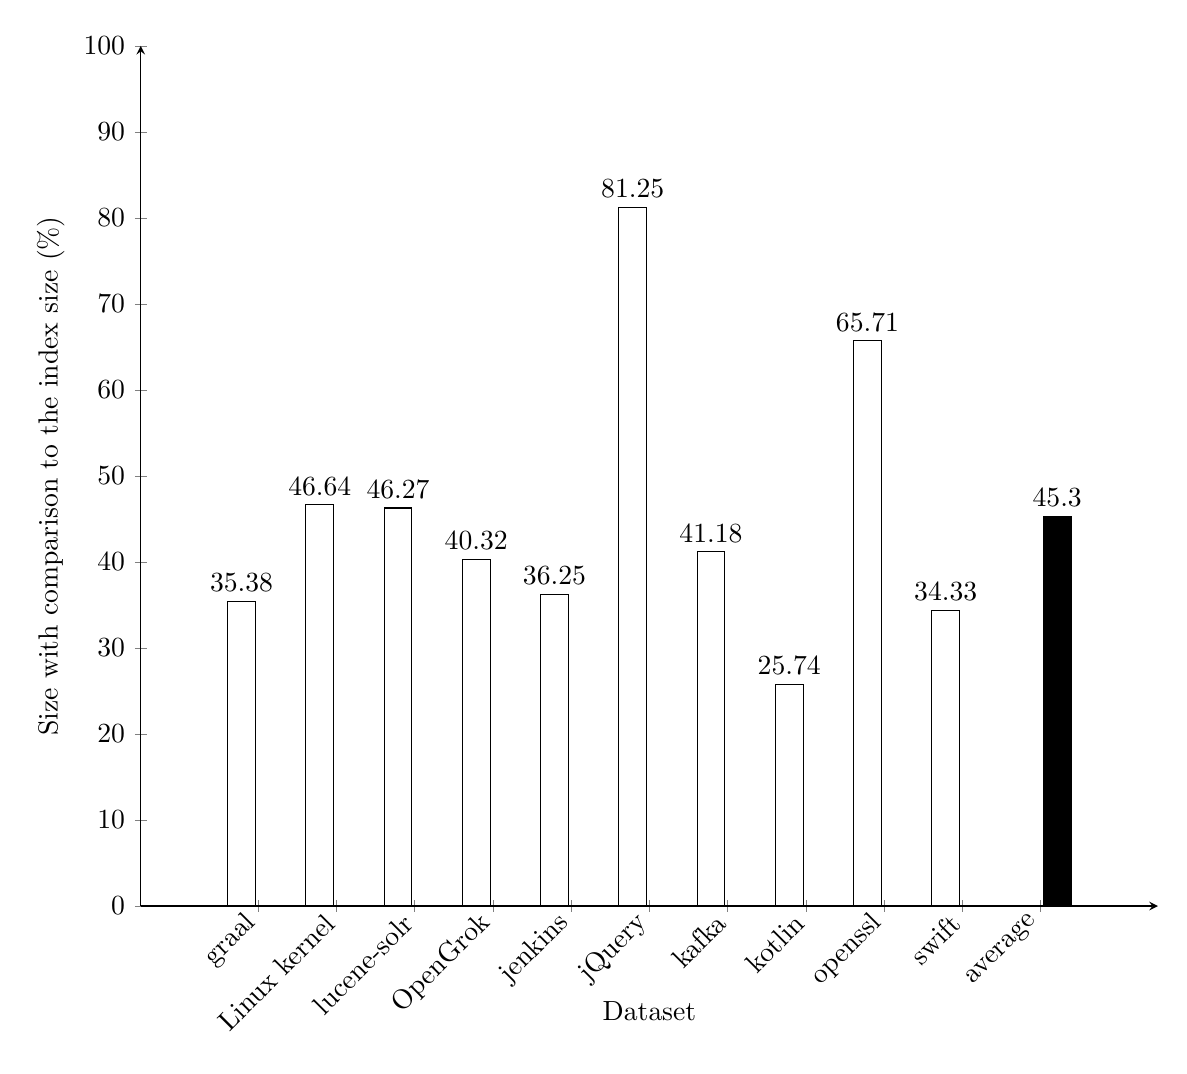
\begin{tikzpicture}
            \begin{axis}[
                width=145mm,
                ybar,
                xlabel={Dataset},
                ylabel={Size with comparison to the index size (\%)},
                ymin=0,
                ymax=100,
                xtick={graal, jenkins, jQuery, kafka, kotlin, Linux kernel, lucene-solr, OpenGrok, openssl, swift, average},
                axis x line=bottom,
                axis y line=left,
                x label style={at={(axis description cs:0.5,-0.1)}},
                enlarge x limits=0.15,
                symbolic x coords={graal, Linux kernel, lucene-solr, OpenGrok, jenkins, jQuery, kafka, kotlin, openssl, swift, average},
                x tick label style={rotate=45,anchor=east},
                nodes near coords={\pgfmathprintnumber\pgfplotspointmeta}
            ]
            \addplot[ybar, fill=white] plot coordinates {
            (graal, 35.38)
            (jenkins, 36.25)
            (jQuery, 81.25)
            (kafka, 41.18)
            (kotlin, 25.74)
            (Linux kernel, 46.64)
            (lucene-solr, 46.27)
            (OpenGrok, 40.32)
            (openssl, 65.71)
            (swift, 34.33)
            };
            \addplot[ybar, fill=black] plot coordinates {
            (average, 45.30)
            };
            \end{axis}
        \end{tikzpicture}
        \caption{Comparison of suggester data size with index size}
        \label{comp_suggester_size}
    \end{figure}

    Projects mentioned on the graph \ref{comp_suggester_size} were:
    \begin{itemize}
        \item \textbf{graal} – \url{https://github.com/oracle/graal}
        \item \textbf{jenkins} – \url{https://github.com/jenkinsci/jenkins}
        \item \textbf{jQuery} – \url{https://github.com/jquery/jquery}
        \item \textbf{kafka} – \url{https://github.com/apache/kafka}
        \item \textbf{kotlin} – \url{https://github.com/JetBrains/kotlin}
        \item \textbf{Linux kernel} – \url{https://github.com/torvalds/linux}
        \item \textbf{lucene-solr} – \url{https://github.com/apache/lucene-solr}
        \item \textbf{OpenGrok} – \url{https://github.com/oracle/opengrok}
        \item \textbf{openssl} – \url{https://github.com/openssl/openssl}
        \item \textbf{swift} – \url{https://github.com/apple/swift}
    \end{itemize}
\end{itemize}

\section{Impact on the Demo Instance}
For monitoring the impact of the suggester, a demo instance was created which can be accessed on the url
\url{http://demo.opengrok.org}. This instance contains 5 projects:
\begin{itemize}
    \item \textbf{elasticsearch}\footnote{\url{https://github.com/elastic/elasticsearch}} – scalable search engine built
    upon Apache Lucene.
    \item \textbf{NetBeans}\footnote{\url{https://github.com/apache/incubator-netbeans}} – NetBeans IDE in development
    under ASF\footnote{\url{https://en.wikipedia.org/wiki/Apache\_Software\_Foundation}}.
    \item \textbf{IntelliJ IDEA Community Edition}\footnote{\url{https://github.com/JetBrains/intellij-community}} –
    open-source edition of the popular IDE.
    \item \textbf{Lucene/Solr}\footnote{\url{https://github.com/apache/lucene-solr}} – combined repository for Apache
    Lucene and Apache Solr.
    \item \textbf{OpenGrok}
\end{itemize}
However, real instances may and often do contain more projects.

The demo instance uses Apache Tomcat servlet container. Many solutions exist which provide a possibility to monitor
applications in a Tomcat instance. From those the most significant are:
\begin{itemize}
    \item \textbf{JMX\footnote{\url{https://en.wikipedia.org/wiki/Java\_Management\_Extensions}} remote} –
    Tomcat provides possiblity to manage and monitor the applications via JMX. Many applications use this functionality
    to their advantage.
    \item \textbf{JavaMelody}\footnote{\url{https://github.com/javamelody/javamelody}} – can be added to the project as a
    dependency and creates a simple page with monitoring information available at \textit{application\_URI/monitoring}.
    Provides monitoring of CPU, memory usage, HTTP requests count and many others. Also allows exporting data in
    various formats, e.g. PDF, JSON. The main disadvantage is that it is embedded into the application and may influence
    the gathered data. However, this overhead is small, e.g. the memory overhead did not exceed 3MiB.
    \item \textbf{PSI Probe}\footnote{\url{https://psi-probe.github.io/psi-probe/}} – deployed as a separate
    application into the Apache Tomcat instance. Uses JMX exported by Tomcat. The disadvantages are:
    \begin{itemize}
        \item Cannot export data in common exchange formats. However, raw XML data are created under the Tomcat
        home directory.
        \item Data are not persistent.
    \end{itemize}
\end{itemize}

\textbf{Chosen solution} JavaMelody was chosen because of its simplicity and because it provided all the needed
features despite the small overhead.

\subsection{Disk Usage}
The demo instance is running on a machine with Linux operating system. Therefore, Chronicle Map takes an advantage of
lazy page allocation and the sizes are significantly smaller in comparison with the sizes on the graph \ref{comp_suggester_size}.
The actual disk usage can be seen on the graph \ref{comp_suggester_size_demo}.
It should be noted that the Chronicle Maps were almost empty.
Similar sizes might be expected as on \ref{comp_suggester_size} if the Chronicle Maps start to fill up.

\begin{figure}[htbp]
    \centering
    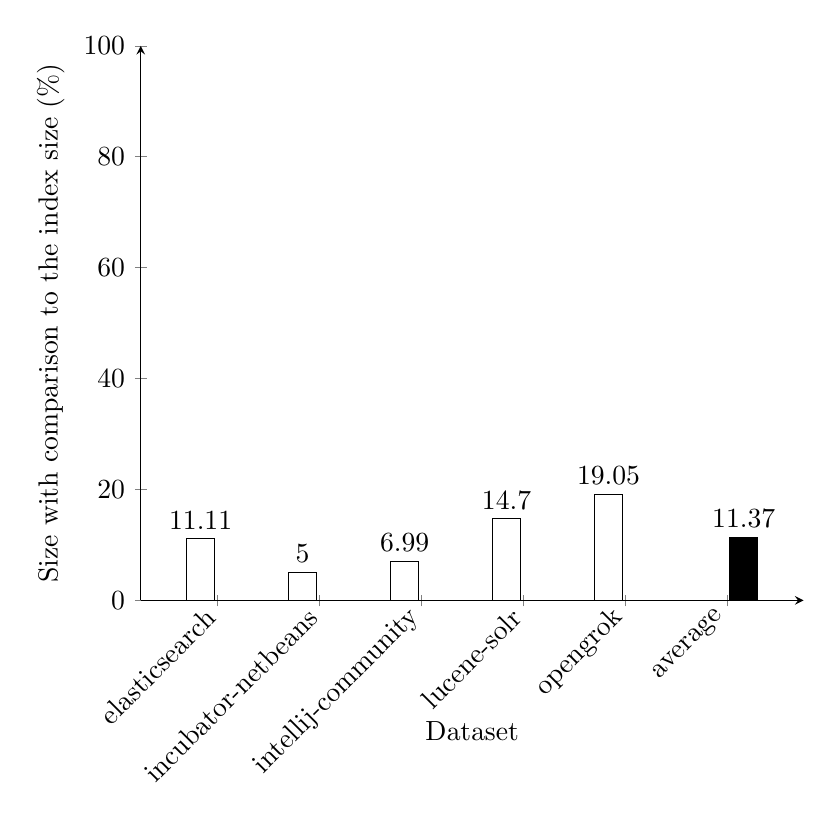
\begin{tikzpicture}
        \begin{axis}[
            width=100mm,
            ybar,
            xlabel={Dataset},
            ylabel={Size with comparison to the index size (\%)},
            ymin=0,
            ymax=100,
            xtick={elasticsearch, incubator-netbeans, intellij-community, lucene-solr, opengrok, average},
            axis x line=bottom,
            axis y line=left,
            x label style={at={(axis description cs:0.5,-0.2)}},
            enlarge x limits=0.15,
            symbolic x coords={elasticsearch, incubator-netbeans, intellij-community, lucene-solr, opengrok, average},
            x tick label style={rotate=45,anchor=east},
            nodes near coords={\pgfmathprintnumber\pgfplotspointmeta}
        ]
        \addplot[ybar, fill=white] plot coordinates {
        (elasticsearch, 11.11)
        (incubator-netbeans, 5.00)
        (intellij-community, 6.99)
        (lucene-solr, 14.70)
        (opengrok, 19.05)
        };
        \addplot[ybar, fill=black] plot coordinates {
        (average, 11.37)
        };
        \end{axis}
    \end{tikzpicture}
    \caption{Comparison of suggester data size with index size on demo instance}
    \label{comp_suggester_size_demo}
\end{figure}
